\section{Versuch 9: VHDL: Demodulator}
	\develnote{Das Quadrat des Signals bilden}

Im Folgenden soll wie auf Seite \pageref{fig:Quadriertessig} beschrieben, die H�llkurvendemodulation in VHDL durchgef�hrt werden. Hierzu m�ssen sie die Ausgangssignale der beiden Bandp�sse quadrieren.

\paragraph{Aufgabe 1:}

Implementieren sie die Quadrierung so, dass die Hardware wieder mehrfach genutzt wird, aber achten Sie darauf, dass nur die ben�tigten Berechnungen durchgef�hrt werden und in den �brigen Zyklen keine unn�tigen Schaltvorg�nge auftreten, da dies nur zu einer erh�hten Stromaufnahme und somit zu unn�tiger Verlustleistung f�hrt.

Verwenden sie die Struktur aus Abbildung \ref{fig:quadschema}

\begin{figure}[hb]
	\centering
		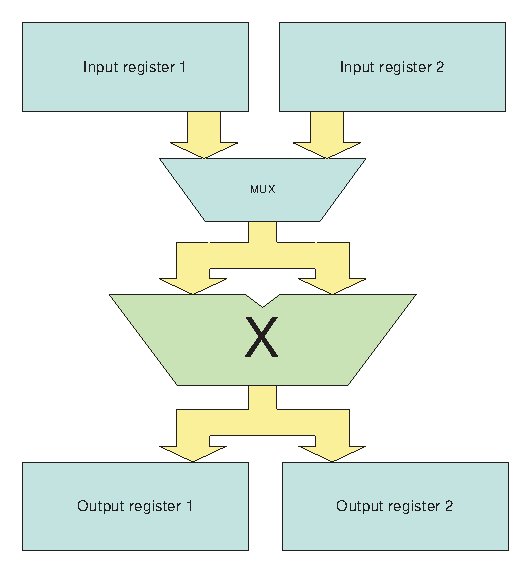
\includegraphics{bilder/empfaenger/quadratur.eps}
	\caption{Quadrierungsschema}
	\label{fig:quadschema}
\end{figure}
